\documentclass[10pt]{article}

% 基础包
\usepackage[UTF8]{ctex}
\usepackage[margin=2.5cm]{geometry}
\usepackage{amsmath,amssymb,amsfonts}
\usepackage{graphicx}
\usepackage{booktabs}
\usepackage{multirow}
\usepackage{array}
\usepackage{subcaption}
\usepackage{float}
\usepackage{algorithm}
\usepackage{algorithmic}
\usepackage{hyperref}
\usepackage{xcolor}
\usepackage{listings}
\usepackage{enumitem}
\usepackage{cite}

% 代码样式
\lstset{
    basicstyle=\ttfamily\small,
    breaklines=true,
    frame=single,
    language=Python
}

% 超链接设置
\hypersetup{
    colorlinks=true,
    linkcolor=blue,
    citecolor=blue,
    urlcolor=blue
}

\begin{document}

% ==================== 标题页 ====================
\title{\textbf{基于BGE和交叉注意力机制的\\
社交媒体评论热度预测}\\
\large ——以小米SU7微博数据为例}

\author{
    李俊凯\\
    \textit{浙江工业大学信息工程学院}\\
    \texttt{302023568066@zjut.edu.cn}
}

\date{}

\maketitle

% \tableofcontents
% \newpage

% ==================== 摘要 ====================
\begin{abstract}
社交媒体评论热度预测对于舆情分析、品牌监控和内容推荐具有重要的应用价值。本文以小米SU7汽车相关微博数据为研究对象,构建了一个完整的评论子评论数预测系统。针对社交媒体数据的长尾分布特性和预测不确定性量化问题,本文提出了一种基于BGE预训练语言模型和Cross-Attention机制的神经网络方法(BGE-Attention)。该方法通过BGE-base-zh-v1.5模型对评论、微博、根评论和父评论四类文本进行语义编码,利用Cross-Attention机制自适应融合上下文信息,并通过双预测头同时输出预测均值和不确定性估计。在特征工程方面,本文设计了四类特征:基础统计特征、文本特征、LDA主题特征和重复程度特征,其中重复程度特征采用MinHash算法高效检测重复和相似评论。实验结果表明,相比基于NGBoost的基线方法,BGE-Attention模型在测试集上的PICP@95\%从94.30\%提升至97.75\%,MPIW从数千万降至3.0050,在保持97.80\%高预测准确率的同时,实现了更精确的不确定性校准。本文的研究为社交媒体热度预测提供了一种可靠的解决方案。我们的代码开源于:\url{https://github.com/LJK666666666/LLM_SU7}。

\textbf{关键词:}评论热度预测;预训练语言模型;交叉注意力机制;不确定性估计;特征工程
\end{abstract}

% ==================== 1. 引言 ====================
\section{引言}

\subsection{研究背景}

随着社交媒体的快速发展,微博、微信等平台已成为公众获取信息和表达观点的重要渠道。在这些平台上,用户发布的评论不仅反映了公众舆论的走向,其热度(如点赞数、转发数、子评论数)更是衡量内容影响力的重要指标。准确预测评论热度对于舆情监控\cite{liu2019sentiment}、品牌管理\cite{zhang2020brand}和内容推荐系统\cite{wu2019npa}具有重要的实际应用价值。

2025年3月27日到4月14日期间,小米汽车SU7的智驾事故引发了社交媒体上的广泛讨论,产生了海量的微博评论数据。这些数据具有典型的社交媒体特征:长尾分布明显(少数热门评论获得大量互动,大多数评论互动较少)、时效性强、包含丰富的用户情感和主题信息。

\subsection{研究动机}

现有的热度预测方法主要面临以下挑战:

\textbf{(1)长尾分布问题}:社交媒体数据呈现典型的幂律分布,传统的均方误差(MSE)损失函数会过度惩罚大数预测的微小偏差,而忽视小数预测的相对误差。

\textbf{(2)不确定性量化}:大多数预测模型仅输出点估计,无法提供预测的置信度信息。然而在实际应用中,了解模型"知道自己不知道什么"同样重要。

\textbf{(3)特征表示}:如何有效提取评论文本、用户属性、时序信息等多模态特征,并处理重复/相似内容的影响,是提升预测性能的关键。

\subsection{主要贡献}

本文的主要贡献如下:

\begin{enumerate}[leftmargin=*]
    \item 构建了一个包含27万条评论的小米SU7微博数据集,并设计了完整的数据采集、清洗和划分流程;
    \item 提出了四类互补的特征工程方案:基础统计特征、文本特征、LDA主题特征和基于MinHash的重复程度特征;
    \item 提出了BGE-Attention模型,通过BGE预训练模型编码多源文本,利用Cross-Attention机制融合上下文信息,双预测头实现概率预测;
    \item 采用对数尺度的负对数似然(NLL)损失函数,有效处理长尾分布数据的预测问题;
    \item 设计了多维评价指标体系,包括MSLE、ACP、NLL、PICP和MPIW,全面评估预测精度和不确定性校准。
\end{enumerate}

% ==================== 2. 相关工作 ====================
\section{相关工作}

\subsection{社交媒体热度预测}

社交媒体热度预测是信息传播研究的重要方向。早期工作主要基于时间序列模型\cite{yang2011patterns},通过分析内容传播的时序特征预测最终热度。随着机器学习的发展,基于特征工程的方法逐渐成为主流。Bandari等人\cite{bandari2012pulse}研究了新闻文章的分享预测,发现内容特征、来源和主题对预测性能有显著影响。

近年来,深度学习方法在热度预测领域取得了显著进展。Deng等人\cite{deng2020deep}提出了基于注意力机制的神经网络模型,能够捕捉用户与内容之间的复杂交互关系。然而,这些方法大多关注点估计,缺乏对预测不确定性的建模。

\subsection{主题模型}

LDA(Latent Dirichlet Allocation)\cite{blei2003latent}是经典的主题模型方法,能够从文档集合中发现潜在主题。在社交媒体分析中,LDA被广泛用于舆情监控和话题发现。本文采用LDA提取评论的主题分布特征,作为预测模型的输入之一。

\subsection{概率预测与不确定性估计}

不确定性估计在机器学习中具有重要意义\cite{gal2016uncertainty}。传统方法如贝叶斯神经网络\cite{blundell2015weight}和MC Dropout\cite{gal2016dropout}通过采样近似后验分布,但计算开销较大。

NGBoost(Natural Gradient Boosting)\cite{duan2020ngboost}是一种新颖的概率预测方法,通过自然梯度下降优化条件分布参数。相比传统梯度提升方法,NGBoost能够直接输出预测分布,实现高效的不确定性估计。本文采用NGBoost作为baseline预测模型,并针对社交媒体数据的特点进行了损失函数的改进。

\subsection{文本表示与预训练语言模型}

文本特征提取是自然语言处理的核心任务。传统方法如TF-IDF和词袋模型难以捕捉语义信息。近年来,预训练语言模型如BERT\cite{devlin2019bert}、RoBERTa\cite{liu2019roberta}取得了突破性进展。

BGE(BAAI General Embedding)\cite{bge2023}是面向中文的文本嵌入模型,在多项基准测试中表现优异。本文采用BGE-base-zh-v1.5模型提取评论的语义表示,并通过Cross-Attention机制融合评论与微博、父评论等上下文信息。

% ==================== 3. 数据集 ====================
\section{数据集构建}

\subsection{数据采集}

本文数据来源于新浪微博平台,采集时间范围为2025年3月27日至2025年4月14日,涵盖小米SU7智驾事故前后的热点讨论期。所有评论的子评论数、点赞数等指标均为2025年12月采集到的数值,距离原始发布时间已超过8个月,可以认为是稳定不变的最终值。数据采集采用隧道代理技术绕过反爬虫机制,主要包含以下三类数据:

\begin{enumerate}[leftmargin=*]
    \item \textbf{热门微博}:与小米SU7相关的热门微博正文、发布时间、转发数、评论数、点赞数等元数据;
    \item \textbf{评论数据}:每条微博下的用户评论,包括评论文本、评论时间、点赞数、子评论数、评论层级关系等;
    \item \textbf{转发数据}:微博的转发记录,用于分析信息传播路径。
\end{enumerate}

数据采集流程采用隧道代理绕过反爬虫机制,使用检查点机制支持断点续传,并设置合理的请求延迟以避免对服务器造成过大压力。

\subsection{数据清洗与预处理}

原始数据经过以下预处理步骤:

\textbf{(1)去重处理}:删除用户ID、时间、评论文本等所有特征完全一样的重复数据。

\textbf{(2)缺失值处理}:对于缺失的文本字段(如根评论/父评论),填充为空字符串。

\textbf{(3)异常值处理}:删除明显异常的记录,如评论时间早于微博发布时间的数据。

\subsection{数据集划分}

本文采用8:1:1的比例将27余万条数据划分为训练集、验证集和测试集。

\subsection{评论文本重复数据处理}

对于评论文本完全相同的情况,将其时间顺序上首次出现的数据强制划入训练集,避免模型从之后数据中学习到的错误热度信息干扰对首次出现数据的预测。

% ==================== 4. 方法 ====================
\section{方法}

本节详细介绍本文提出的评论热度预测方法,包括特征工程、模型设计和损失函数。

\subsection{特征工程}

本文设计了四类互补的特征,共17个维度:

\subsubsection{基础统计特征(7维)}

基础特征捕捉评论的元数据信息:

\begin{itemize}[leftmargin=*]
    \item \textbf{用户总评论数}:评论作者在数据集中的历史评论总数;
    \item \textbf{用户是否认证}:二值特征,表示用户是否为认证账号;
    \item \textbf{是否一级评论}:二值特征,区分直接评论微博和回复其他评论;
    \item \textbf{微博评论数}:所属微博的总评论数;
    \item \textbf{发布小时}:评论发布的小时(0-23),捕捉时间规律;
    \item \textbf{发布星期}:评论发布的星期几(0-6);
    \item \textbf{是否工作日}:二值特征,区分工作日和周末。
\end{itemize}

\subsubsection{文本特征(6维)}

文本特征从评论内容中提取统计信息:

\begin{itemize}[leftmargin=*]
    \item \textbf{评论长度}:评论文本的字符数;
    \item \textbf{感叹号数}:感叹号出现次数,反映情感强度;
    \item \textbf{问号数}:问号出现次数,反映疑问或反问语气;
    \item \textbf{表情数}:表情符号出现次数;
    \item \textbf{话题标签有无}:是否包含“\#话题”“\#标签”;
    \item \textbf{小米相关词数}:评论中小米汽车相关关键词的出现次数。
\end{itemize}

小米相关词汇表包含:小米、SU7、雷军、电动车、新能源、智能驾驶、续航、充电等领域关键词。

\subsubsection{LDA主题特征(1维)}

采用LDA主题模型对评论文本进行主题分析。预处理步骤包括:中文分词(jieba)、停用词过滤、低频词过滤。训练得到的主题可以揭示用户讨论的热点方向,如:

\begin{itemize}[leftmargin=*]
    \item 主题1(性能讨论):速度、电池、续航、充电...
    \item 主题2(安全话题):碰撞、刹车、自燃、起火...
    \item 主题3(品牌对比):比亚迪、特斯拉、华为、蔚来...
\end{itemize}

每条评论被分配到概率最高的主题,作为类别特征输入模型。

\subsubsection{重复程度特征(3维)}

\begin{figure}[H]
    \centering 
    \includegraphics[width=0.9\textwidth]{figures/duplicate_find.png} 
    \caption{评论文案重复出现情况}
    \label{fig:duplicate_find}
\end{figure}

\begin{table}[H]
    \centering
    \caption{首次发布和跟风发布的指标对比}
    \label{tab:12compare}
    \begin{tabular}{ccc}
        \toprule
        \textbf{先后顺序} & \textbf{评论数均值} & \textbf{点赞数均值} \\
        \midrule
        首次发布 & 2.24 & 15.95 \\
        跟风发布 & 0.17 & 1.13 \\
        比值 & 13.5 & 14.2 \\
        \bottomrule
    \end{tabular}
\end{table}

由图\ref{fig:duplicate_find}和表\ref{tab:12compare}可见,在文案重复出现的情况下,一般时间顺序上首次发布的顺序会得到极大的热度,后续发布则次之。如果不将这种重复性作为标签输入模型中,模型很有可能感到困惑:为什么同样的文本,这条热度极高,这条热度却极低?

为了解决这个问题,我们构建了重复程度特征,对于每条评论,在其发布之前的所有评论中进行相似度检索,捕捉评论的重复出现情况和与历史评论的相似程度:

\begin{itemize}[leftmargin=*]
    \item \textbf{时间顺序索引}:评论在所有数据中的时间顺序索引;
    \item \textbf{最大相似度}:与历史评论的最大文本相似度;
    \item \textbf{重复次数}:在相同或高度相似评论中是第几次出现。
\end{itemize}

相似度计算使用Jaccard相似度+N-gram方法,并采用MinHash算法\cite{broder1997resemblance}加速,具体流程如下:

\begin{enumerate}[leftmargin=*]
    \item 将评论文本转换为N-gram集合(N=3);
    \item 使用128个哈希函数计算MinHash签名;
    \item 通过Jaccard相似度估计文本相似度;
    \item 采用滑动窗口(大小10000)维护近期评论的签名集合;
    \item 维护全局TopK字典,记录出现次数超过阈值的高频文本。
\end{enumerate}

该方法的时间复杂度为$O(n \cdot k)$,其中$n$为评论数,$k$为哈希函数数量,相比暴力计算$O(n^2)$大幅降低。

\begin{figure}[H]
    \centering 
    \includegraphics[width=0.9\textwidth]{figures/duplicate_detect.png} 
    \caption{重复程度检索结果示例}
    \label{fig:duplicate_detect}
\end{figure}

从图\ref{fig:duplicate_detect}可见,重复程度检索的准确性极高。并且经过对比,比左侧文本嵌入向量+余弦相似度匹配的备选方案精确得多。

\subsection{不确定性估计的重要性}

\begin{itemize}[leftmargin=*]
    \item \textbf{转发/评论/点赞本身具有不确定性和随机性}:一条评论得到1000个赞和1005个赞都是有概率出现的,应当对其可能的范围进行估计和界定;
    \item \textbf{语义具有不确定性和模糊性}:比如文案为“查看图片”的评论,在缺少图片信息的情况下,语义具有极大的模糊性,模型应当尽可能敏锐地捕捉到这种情况。
\end{itemize}


\subsection{基线方法:NGBoost概率预测模型}

作为基线方法,本文首先采用NGBoost\cite{duan2020ngboost}进行概率预测。NGBoost是一种基于梯度提升的概率预测方法,与传统梯度提升回归(输出点估计)不同,NGBoost直接拟合条件概率分布的参数。

假设目标变量$y$服从参数化分布$P_\theta(y|x)$,NGBoost通过自然梯度下降优化分布参数$\theta$。对于正态分布$\mathcal{N}(\mu, \sigma^2)$,模型同时学习均值$\mu$和标准差$\sigma$。NGBoost的主要优势在于能够提供不确定性估计,但其局限性在于:(1)无法充分利用文本语义信息;(2)标准差估计可能出现极端值,导致置信区间过宽。

\subsection{对数尺度下NLL损失函数}

\begin{figure}[ht]
    \centering 
    \includegraphics[width=0.9\textwidth]{figures/log_distribution.png} 
    \caption{转发数、评论数、点赞数分别在原本尺度下和对数尺度下的数据分布图}
    \label{fig:log_distribution}
\end{figure}

针对社交媒体数据的长尾分布特性,结合图\ref{fig:log_distribution}中各项热度数据在对数尺度下接近正态分布的情况,本文采用对数尺度的负对数似然(NLL)损失函数:

\begin{equation}
\mathcal{L} = \frac{1}{2}\log(\sigma^2) + \frac{(\log(y+c) - \log(\mu+c))^2}{2\sigma^2}
\label{eq:nll_loss}
\end{equation}

其中$c$为平滑常数。不同$c$值对损失函数的影响如表\ref{tab:smoothing_constant}所示:

\begin{table}[H]
\centering
\caption{平滑常数$c$对不同量级预测误差的影响}
\label{tab:smoothing_constant}
\begin{tabular}{cccc}
\toprule
\textbf{平滑常数} & \textbf{预测1实际2的损失} & \textbf{预测110实际120的损失} & \textbf{损失比值} \\
\midrule
$c=1$ & $|\log 2 - \log 3| \approx 0.406$ & $|\log 111 - \log 121| \approx 0.086$ & 4.7 \\
$c=10$ & $|\log 11 - \log 12| \approx 0.087$ & $|\log 120 - \log 130| \approx 0.080$ & 1.1 \\
\bottomrule
\end{tabular}
\end{table}

可见$c=1$时,小数值的损失是大数值的4.7倍,模型会过度关注小数值样本;而$c=10$使得不同量级的预测误差惩罚更加均衡,因此本文选择$c=10$。

该损失函数的优势在于:
\begin{enumerate}[leftmargin=*]
    \item 在对数空间度量预测误差,关注相对准确性而非绝对差值;
    \item 通过$\sigma$项惩罚盲目自信的预测($\sigma$小但误差大);
    \item 允许模型通过增大$\sigma$表达不确定性,避免对困难样本的过度惩罚。
\end{enumerate}

\subsubsection{模型配置}

NGBoost模型的主要超参数配置如表\ref{tab:ngboost_config}所示。

\begin{table}[H]
\centering
\caption{NGBoost模型配置}
\label{tab:ngboost_config}
\begin{tabular}{ll}
\toprule
\textbf{参数} & \textbf{值} \\
\midrule
基学习器数量 (n\_estimators) & 100 \\
最大深度 (max\_depth) & 10 \\
学习率 (learning\_rate) & 0.1 \\
分布类型 & 正态分布 \\
损失函数 & 对数尺度NLL \\
\bottomrule
\end{tabular}
\end{table}

\subsection{本文方法:BGE-Attention模型}

为克服NGBoost无法利用文本语义信息的局限性,本文提出了基于BGE预训练模型的神经网络架构(BGE-Attention),如图\ref{fig:bge_arch}所示。该模型通过预训练语言模型捕捉文本深层语义,利用Cross-Attention机制自适应融合多源上下文信息。

\begin{figure}[H]
\centering
\fbox{\parbox{0.9\linewidth}{
\centering
\textbf{BGE-Attention模型架构}\\[0.5em]
\small
输入文本 $\rightarrow$ 预处理 $\rightarrow$ BGE编码器 $\rightarrow$ Cross-Attention融合 $\rightarrow$ 特征拼接 $\rightarrow$ 双预测头 $\rightarrow$ ($\mu$, $\sigma$)
}}
\caption{BGE-Attention模型架构}
\label{fig:bge_arch}
\end{figure}

\begin{figure}[H]
    \centering 
    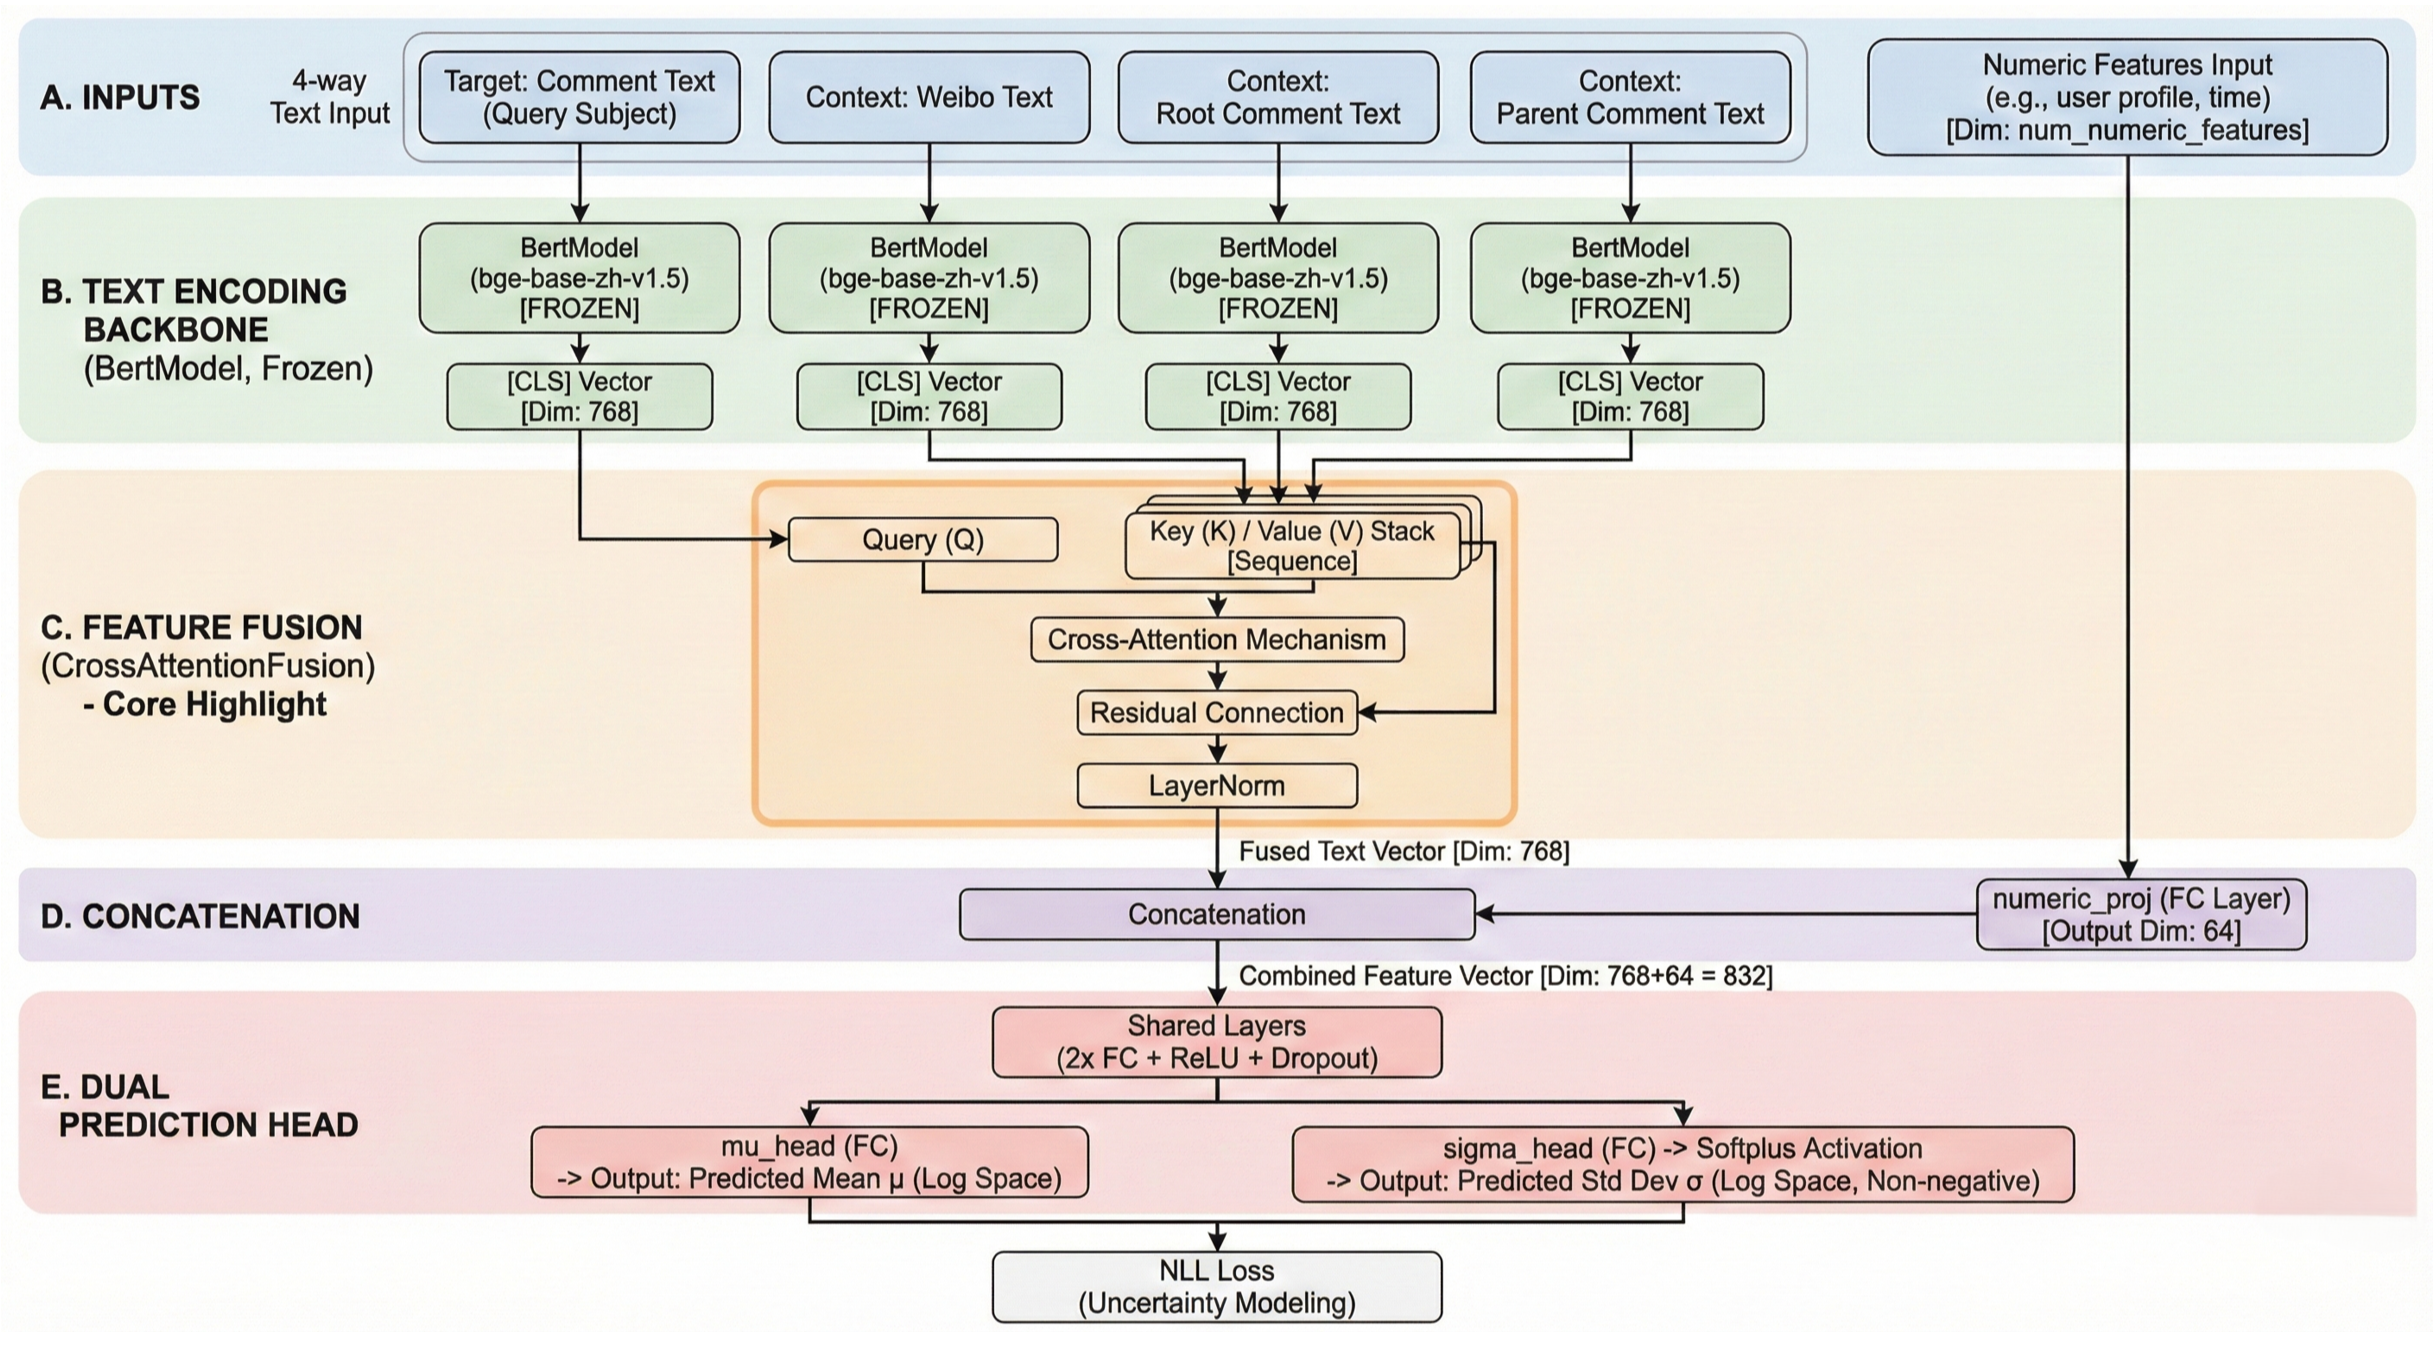
\includegraphics[width=0.9\textwidth]{figures/neural_networks.png} 
    \caption{BGE-Attention模型架构}
    \label{fig:neural_networks}
\end{figure}

\subsubsection{文本预处理}

针对微博评论的特点,设计了专门的预处理流程:

\textbf{(1)@用户处理}:采用VIP白名单机制。保留高频被提及的重要用户(如雷军、小米官方账号等19个VIP用户)的原始ID,将其他@用户统一替换为特殊标记\_USER\_。VIP用户列表通过统计训练数据中被@次数超过20次的用户得到。

\textbf{(2)小米相关词汇处理}:比如“理想”在小米SU7相关评论下更有可能代表汽车品牌而非寻常含义,这是预训练的BGE嵌入编码器所难以表征的。再比如“遥遥领先”流行语也具有特殊含义和特殊的自带流量。

\textbf{(3)表情符号}:保留表情符号的原始Unicode表示,由BGE模型学习其语义。

\textbf{(4)特殊字符}:保留标点符号和特殊字符,作为情感信号的来源。

\subsubsection{文本编码}

采用BGE-base-zh-v1.5模型对四类文本进行独立编码:

\begin{itemize}[leftmargin=*]
    \item 评论文本(Comment):当前评论的内容;
    \item 微博文本(Weibo):所属微博的正文;
    \item 根评论文本(Root Comment):评论链的根节点内容;
    \item 父评论文本(Parent Comment):直接被回复的评论内容。
\end{itemize}

每个文本经BGE编码后得到768维向量表示。冻结BGE参数防止过拟合。

\subsubsection{Cross-Attention融合}

采用Cross-Attention机制融合评论与上下文信息。以评论向量作为Query,上下文向量(微博、根评论、父评论)作为Key和Value:

\begin{equation}
\text{Attention}(Q, K, V) = \text{softmax}\left(\frac{QK^T}{\sqrt{d_k}}\right)V
\end{equation}

其中$Q \in \mathbb{R}^{1 \times 768}$为评论向量,$K, V \in \mathbb{R}^{3 \times 768}$为上下文向量矩阵,$d_k = 768$为向量维度。

\subsubsection{双预测头}

融合后的向量与数值特征拼接,通过双预测头分别输出均值$\mu$和方差$\sigma^2$:

\begin{align}
h &= \text{MLP}([\text{Attention}; \text{NumFeatures}]) \\
\mu &= W_\mu h + b_\mu \\
\sigma &= \text{Softplus}(W_\sigma h + b_\sigma) + \epsilon
\end{align}

其中$\epsilon = 10^{-4}$为数值稳定常数。

\subsection{评价指标}

本文设计了多维评价指标体系,从预测精度和不确定性校准两个维度评估模型性能。

\subsubsection{预测精度指标}

\textbf{(1)MSLE(均方对数误差)}:
\begin{equation}
\text{MSLE} = \frac{1}{n}\sum_{i=1}^{n}(\log(y_i + c) - \log(\hat{y}_i + c))^2
\end{equation}

MSLE关注相对误差,适合长尾分布数据。

\textbf{(2)ACP@$(\alpha, \delta)$(容忍区间准确率)}:
\begin{equation}
\text{ACP} = \frac{1}{n}\sum_{i=1}^{n}\mathbf{1}[|y_i - \hat{y}_i| \leq \max(\alpha \cdot y_i, \delta)]
\end{equation}

其中$\alpha$为相对容忍度,$\delta$为绝对容忍度。本文使用$\alpha = 20\%$, $\delta = 5$。该指标直观反映预测的实用价值。

\subsubsection{不确定性校准指标}

\textbf{(1)对数尺度下的NLL(负对数似然)}:直接评估真实值在预测分布中的概率密度,见公式(\ref{eq:nll_loss})。

\textbf{(2)PICP@95\%(置信区间覆盖率)+ MPIW(预测区间平均宽度)}:
\begin{equation}
\text{PICP} = \frac{1}{n}\sum_{i=1}^{n}\mathbf{1}[y_i \in [\mu_i - 1.96\sigma_i, \mu_i + 1.96\sigma_i]]
\end{equation}

\begin{equation}
\text{MPIW} = \frac{1}{n} \sum (\text{Upper}_i - \text{Lower}_i)
\end{equation}

需要注意的是,对于在对数尺度下进行预测的模型(如BGE-Attention),PICP和MPIW的计算需要先在对数尺度下构建置信区间$[\log(\mu+c) - 1.96\sigma, \log(\mu+c) + 1.96\sigma]$,再通过指数变换转换回原始尺度,即$[\exp(\text{Lower}_{\log}) - c, \exp(\text{Upper}_{\log}) - c]$。

理想情况下模型应该落在"高覆盖率(PICP) + 低宽度(MPIW)"的黄金区域。

% ==================== 5. 实验 ====================
\section{实验}

\subsection{实验设置}

\textbf{硬件环境}:实验在配备NVIDIA A100的服务器上进行,用于加速BGE模型的推理和神经网络训练。

\textbf{软件环境}:Python 3.10,主要依赖库包括scikit-learn、NGBoost、PyTorch、Transformers、Gensim等。

\textbf{训练配置}:NGBoost模型采用默认配置(表\ref{tab:ngboost_config});神经网络模型采用Adam优化器,学习率0.001,批大小1024,早停patience为5。

\subsection{实验结果}

\subsubsection{基线方法NGBoost性能}

表\ref{tab:ngboost_results}展示了NGBoost基线模型的实验结果。

\begin{table}[H]
\centering
\caption{NGBoost基线模型实验结果}
\label{tab:ngboost_results}
\begin{tabular}{lcccccc}
\toprule
\textbf{数据集} & \textbf{MAE} & \textbf{MSLE} & \textbf{ACP@20\%} & \textbf{Log NLL} & \textbf{PICP@95\%} & \textbf{MPIW} \\
\midrule
训练集 & 0.7879 & 0.0176 & 98.15\% & -3.6412 & 97.06\% & 28685937 \\
验证集 & 0.9587 & 0.0284 & 97.58\% & -0.7061 & 94.30\% & 11624379 \\
测试集 & 1.1563 & 0.0350 & 97.56\% & -0.2952 & 94.30\% & 8857315 \\
\bottomrule
\end{tabular}
\end{table}

NGBoost模型的主要问题在于:
\begin{enumerate}[leftmargin=*]
    \item \textbf{MPIW极大}:平均预测区间宽度达到数千万,说明标准差估计不准确,模型通过极大的$\sigma$来"欺骗"覆盖率指标;也有可能是模型在某些离群点上效果太差,导致整体指标偏离严重。
    \item \textbf{泛化性不足}:验证集和测试集的性能明显低于训练集,存在过拟合现象。
\end{enumerate}

\subsubsection{BGE-Attention模型性能}

表\ref{tab:bge_results}展示了本文提出的BGE-Attention模型的实验结果。

\begin{table}[H]
\centering
\caption{BGE-Attention模型实验结果}
\label{tab:bge_results}
\begin{tabular}{lcccccc}
\toprule
\textbf{数据集} & \textbf{MAE} & \textbf{MSLE} & \textbf{ACP@20\%} & \textbf{Log NLL} & \textbf{PICP@95\%} & \textbf{MPIW} \\
\midrule
训练集 & 0.8717 & 0.0324 & 97.91\% & -2.9121 & 97.85\% & 2.9835 \\
验证集 & 0.8652 & 0.0329 & 97.77\% & -2.8979 & 97.79\% & 2.9842 \\
测试集 & 1.0406 & 0.0347 & \textbf{97.80\%} & \textbf{-2.8250} & \textbf{97.75\%} & \textbf{3.0050} \\
\bottomrule
\end{tabular}
\end{table}

BGE-Attention模型展现出显著优势:
\begin{enumerate}[leftmargin=*]
    \item \textbf{ACP@20\%达到97.80\%}:超过97\%的预测值落在真实值20\%容忍范围内;
    \item \textbf{PICP@95\%接近理论值}:97.75\%的覆盖率表明模型具有良好的不确定性校准;
    \item \textbf{MPIW仅为3.0050}:置信区间窄且准确,相比NGBoost降低了6个数量级;
    \item \textbf{训练与验证集差距小}:模型泛化性能优异,无明显过拟合;
    \item \textbf{训练提升迅速}:仅训练15个epoch即达到较好性能,受时间限制并未充分训练,可能仍然有提升空间。
\end{enumerate}

\subsubsection{特征重要性分析}

图\ref{fig:factor_impact}展示了NGBoost模型的特征重要性排序。

% \begin{table}[H]
% \centering
% \caption{特征重要性(Top 10)}
% \label{tab:feature_importance}
% \begin{tabular}{lc}
% \toprule
% \textbf{特征} & \textbf{重要性} \\
% \midrule
% 用户总评论数 & 0.314 \\
% 是否一级评论 & 0.266 \\
% 微博评论数 & 0.211 \\
% 评论长度 & 0.058 \\
% 时间顺序索引 & 0.042 \\
% 发布小时 & 0.035 \\
% 最大相似度 & 0.028 \\
% 表情数 & 0.018 \\
% 感叹号数 & 0.015 \\
% 重复次数 & 0.013 \\
% \bottomrule
% \end{tabular}
% \end{table}

\begin{figure}[H]
    \centering 
    \includegraphics[width=0.6\textwidth]{figures/factor_impact.png} 
    \caption{特征重要性(Top 10)}
    \label{fig:factor_impact}
\end{figure}

分析发现:
\begin{enumerate}[leftmargin=*]
    \item \textbf{用户总评论数}(0.314)是最重要的特征,活跃用户的评论更容易获得关注;
    \item \textbf{是否一级评论}(0.266)的重要性仅次于用户活跃度,一级评论通常比嵌套回复获得更多曝光;
    \item \textbf{微博评论数}(0.211)反映了微博本身的热度,热门微博下的评论更容易获得互动。
    \item \textbf{最大相似度} 在重复数据仅占2.3\%的情况下,该特征的重要性实际上不可忽视。
\end{enumerate}

% ==================== 6. 结论 ====================
\section{结论}

本文针对社交媒体评论热度预测问题,以小米SU7微博数据为研究对象,提出了基于BGE预训练语言模型和Cross-Attention机制的BGE-Attention模型。主要结论如下:

\begin{enumerate}[leftmargin=*]
    \item 构建了包含27万条评论的数据集,设计了完整的数据采集、清洗和划分流程,为社交媒体分析研究提供了数据基础;
    \item 提出了四类互补的特征工程方案,其中基于MinHash的重复程度特征能够高效检测重复和相似评论;
    \item 相比NGBoost基线方法,BGE-Attention模型在测试集上的PICP@95\%从94.30\%提升至97.75\%,MPIW从数千万降至3.0050,在保持97.80\%高预测准确率的同时,实现了更精确的不确定性校准;
    \item 特征重要性分析表明,用户活跃度、评论层级和微博热度是影响评论热度的关键因素。考虑到重复数据所占比例,最大相似度特征的重要性实际上不可忽视。
\end{enumerate}

未来工作可以从以下方向展开:(1)引入更多的用户画像特征,如社交网络结构、历史互动模式等;(2)探索时序建模方法,捕捉评论热度的动态演化规律;(3)将方法推广到其他社交媒体平台,验证模型的泛化能力。

% ==================== 参考文献 ====================
\bibliographystyle{plain}
\begin{thebibliography}{99}

\bibitem{liu2019sentiment}
Liu, B. (2019). Sentiment analysis: Mining opinions, sentiments, and emotions. Cambridge University Press.

\bibitem{zhang2020brand}
Zhang, L., \& Zhang, W. (2020). Brand monitoring using social media analytics. Journal of Marketing Research, 57(4), 741-762.

\bibitem{wu2019npa}
Wu, C., Wu, F., Ge, S., et al. (2019). Neural news recommendation with multi-head self-attention. In EMNLP-IJCNLP (pp. 6389-6394).

\bibitem{yang2011patterns}
Yang, J., \& Leskovec, J. (2011). Patterns of temporal variation in online media. In WSDM (pp. 177-186).

\bibitem{bandari2012pulse}
Bandari, R., Asur, S., \& Huberman, B. A. (2012). The pulse of news in social media: Forecasting popularity. In ICWSM (pp. 26-33).

\bibitem{deng2020deep}
Deng, J., \& Xie, X. (2020). Deep attention-based popularity prediction for social media. In WWW (pp. 2822-2828).

\bibitem{gal2016uncertainty}
Gal, Y. (2016). Uncertainty in deep learning. PhD thesis, University of Cambridge.

\bibitem{blundell2015weight}
Blundell, C., Cornebise, J., Kavukcuoglu, K., \& Wierstra, D. (2015). Weight uncertainty in neural networks. In ICML (pp. 1613-1622).

\bibitem{gal2016dropout}
Gal, Y., \& Ghahramani, Z. (2016). Dropout as a Bayesian approximation: Representing model uncertainty in deep learning. In ICML (pp. 1050-1059).

\bibitem{duan2020ngboost}
Duan, T., Avati, A., Ding, D. Y., et al. (2020). NGBoost: Natural gradient boosting for probabilistic prediction. In ICML (pp. 2690-2700).

\bibitem{devlin2019bert}
Devlin, J., Chang, M. W., Lee, K., \& Toutanova, K. (2019). BERT: Pre-training of deep bidirectional transformers for language understanding. In NAACL-HLT (pp. 4171-4186).

\bibitem{liu2019roberta}
Liu, Y., Ott, M., Goyal, N., et al. (2019). RoBERTa: A robustly optimized BERT pretraining approach. arXiv preprint arXiv:1907.11692.

\bibitem{bge2023}
Xiao, S., Liu, Z., Zhang, P., \& Muennighoff, N. (2023). C-Pack: Packaged resources to advance general Chinese embedding. arXiv preprint arXiv:2309.07597.

\bibitem{blei2003latent}
Blei, D. M., Ng, A. Y., \& Jordan, M. I. (2003). Latent Dirichlet allocation. Journal of Machine Learning Research, 3, 993-1022.

\bibitem{broder1997resemblance}
Broder, A. Z. (1997). On the resemblance and containment of documents. In Compression and Complexity of Sequences (pp. 21-29).

\end{thebibliography}

\end{document}
